% =============================================================================
\section{Results}
\label{sec:results}
% =============================================================================

\begin{center}
\noteto{Francisco}{This section is yours too -- please fill in the real logs/plots/numbers below once available (from pool/lake/field tests or simulation runs), and add the actual figures in place of the placeholders.}
\end{center}

This section reports closed-loop performance for (i) the decoupled $v$/$w$ velocity controller (Section~\ref{sec:vw}) in isolation, and (ii) the full ILOS trajectory-following stack (Section~\ref{sec:ilos}--\ref{sec:mission}) on the example missions of Table~\ref{tab:missions}. \todored{All figures and numeric values in this section are placeholders. Replace each placeholder box with the corresponding plot (e.g.\ exported from a rosbag via \texttt{rqt\_plot}/\texttt{plotjuggler}/matplotlib) and fill in the tables once logs from the pool/lake/field tests (or simulation runs) are available.}

\subsection{$v$/$w$ tracking performance}

\textbf{Test protocol.} The velocity controller was exercised in \texttt{GUIDED} mode in the Gazebo digital twin (Section~\ref{sec:sim}, \texttt{feup} world, calm water), running the simulation gain set of Table~\ref{tab:pid} (\texttt{velocity\_controller\_sim.yaml}) at the nominal $f_s=50$\,Hz control rate. Three step tests were logged, each holding the commanded setpoint for $15$\,s: (i) an \emph{isolated surge} step $v_{\text{cmd}}:0\to1.0$~m/s with $w_{\text{cmd}}=0$; (ii) an \emph{isolated yaw} step $w_{\text{cmd}}:0\to0.5$~rad/s with $v_{\text{cmd}}=0$; and (iii) a \emph{coupled} step with $v_{\text{cmd}}:0\to0.5$~m/s and $w_{\text{cmd}}:0\to0.5$~rad/s applied simultaneously, to probe the surge/yaw decoupling assumption of Section~\ref{sec:vw}. The fused-odometry measurements $v_{\text{meas}}, w_{\text{meas}}$ were recorded and the metrics of Table~\ref{tab:vwresults} computed from them (settling times evaluated on a lightly smoothed trace so that steady-state odometry ripple is not mistaken for residual transient).

\begin{figure}[H]
\centering
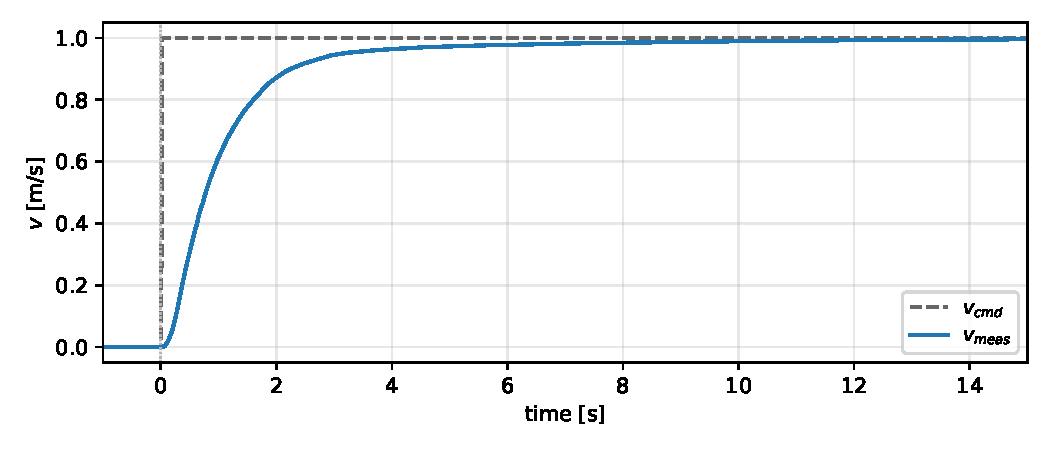
\includegraphics[width=0.9\linewidth]{figures/pid_step_surge.pdf}
\caption{Isolated surge velocity step response ($v_{\text{cmd}}:0\to1.0$~m/s, $w_{\text{cmd}}=0$): fused-odometry $v_{\text{meas}}(t)$ against the commanded step. The response is essentially first-order with no overshoot ($\sim$2\,s rise, $\sim$6.5\,s settling to the 2\% band).}
\label{fig:step_surge}
\end{figure}

\begin{figure}[H]
\centering
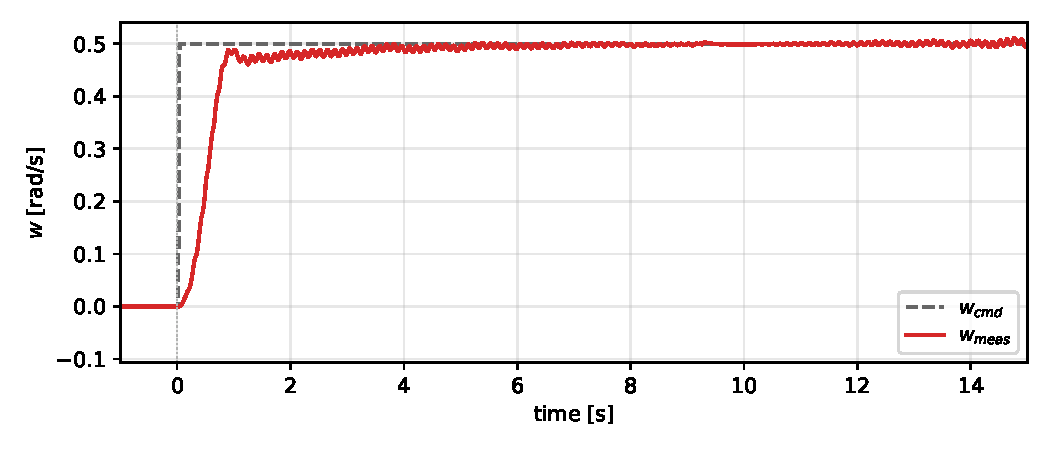
\includegraphics[width=0.9\linewidth]{figures/pid_step_yaw.pdf}
\caption{Isolated yaw-rate step response ($w_{\text{cmd}}:0\to0.5$~rad/s, $v_{\text{cmd}}=0$): $w_{\text{meas}}(t)$ against the commanded step. The yaw loop is markedly faster than surge ($\sim$0.5\,s rise) with a small $\sim$2\% overshoot and negligible steady-state error.}
\label{fig:step_yaw}
\end{figure}

\begin{figure}[H]
\centering
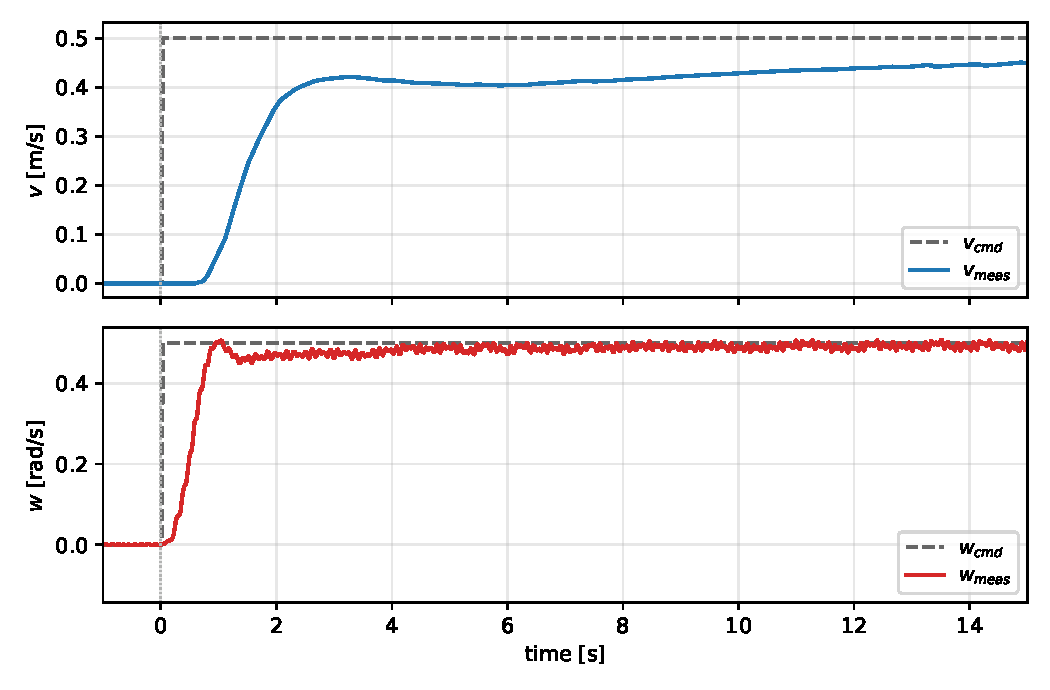
\includegraphics[width=0.9\linewidth]{figures/pid_step_coupled.pdf}
\caption{Coupled step ($v_{\text{cmd}}:0\to0.5$~m/s and $w_{\text{cmd}}:0\to0.5$~rad/s applied together). Yaw tracking (bottom) is essentially unaffected, but surge (top) becomes sluggish and settles $\sim$10\% low: with both a common-mode (surge) and a differential (yaw) thrust demand, one thruster approaches its $\pm T_{\max}$ limit and surge authority is transiently sacrificed to preserve yaw.}
\label{fig:step_coupled}
\end{figure}

\begin{table}[H]
\centering
\caption{Velocity-tracking performance metrics, isolated surge and yaw step tests (Gazebo, simulation gains).}
\label{tab:vwresults}
\begin{tabular}{@{}lcccc@{}}
\toprule
Axis & Rise time (10--90\%) & Overshoot [\%] & Settling time (2\%) & Steady-state error\\
\midrule
Surge $v$ ($0\to1.0$~m/s)  & 2.0\,s & 0.0 & 6.5\,s & $\approx 0.004$~m/s \\
Yaw $w$ ($0\to0.5$~rad/s)  & 0.5\,s & 2.2 & 4.3\,s & $\approx 0.001$~rad/s \\
\bottomrule
\end{tabular}
\end{table}

Both axes track their setpoints with negligible steady-state error, confirming that the integral action (with directional anti-windup, Section~\ref{sec:pid}) removes the residual drag offset. The yaw loop is roughly four times faster than surge, consistent with its much higher proportional gain (Table~\ref{tab:pid}). The coupled test (Figure~\ref{fig:step_coupled}) shows the decoupling assumption holds well for yaw but only approximately for surge under simultaneous large yaw demand, where thruster saturation in the mixer (Eqs.~\eqref{eq:mixL}--\eqref{eq:mixR}) reduces available surge force.

\subsection{Trajectory-following performance}

\textbf{Test protocol.} The full ILOS guidance stack (Section~\ref{sec:ilos}) was run in the Gazebo digital twin on a closed \emph{square} mission: a $40\times40$~m box (waypoints offset $3$~m in East from the spawn point) traversed for $3$ consecutive laps, using the square-mission guidance parameters of Table~\ref{tab:ilosparams} ($k_i=0$, i.e.\ pure LOS, in calm water with no current). The vehicle pose was logged at the $10$~Hz guidance rate; cross-track error $e_y$ and the per-lap/per-leg statistics were computed online by the characterization node.

\begin{figure}[H]
\centering
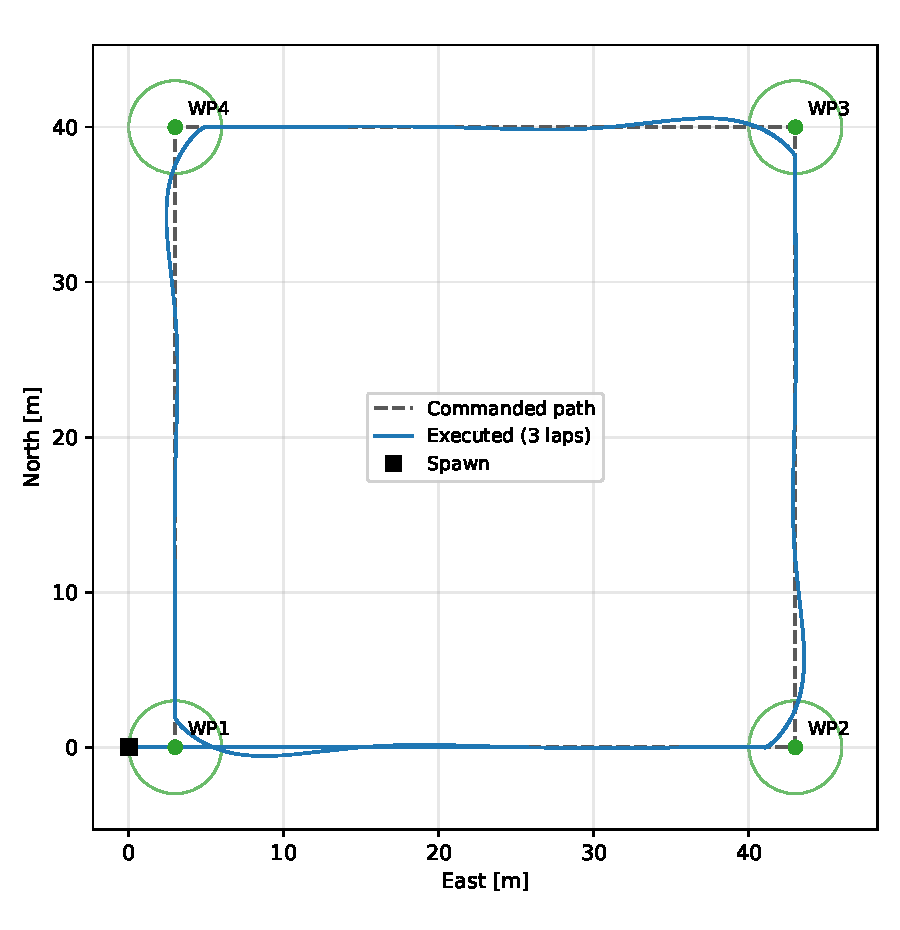
\includegraphics[width=0.72\linewidth]{figures/traj_square_path.pdf}
\caption{Executed path (ENU) over 3 laps against the commanded square. Waypoint markers show the $R_{\text{wp}}=3$~m arrival radius; the vehicle deliberately cuts each corner as it switches to the next leg once inside $R_{\text{wp}}$, so the executed path ($429$~m) is shorter than the ideal polyline ($480$~m).}
\label{fig:traj_path}
\end{figure}

\begin{figure}[H]
\centering
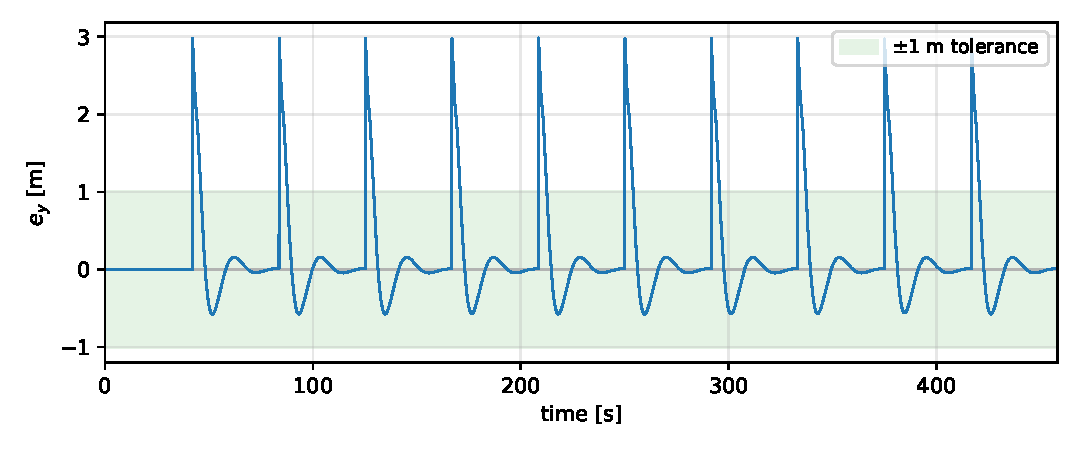
\includegraphics[width=\linewidth]{figures/traj_square_ey.pdf}
\caption{Cross-track error $e_y(t)$ for the square mission. On the straight legs $e_y$ is held to the millimetre level; each of the 11 corners produces a transient spike to $\sim$3~m (the vehicle is momentarily off the \emph{new} leg the instant it switches at the waypoint), which the LOS law rejects within a few seconds with a small ($\sim$0.7~m) undershoot before re-converging. The shaded band is the $\pm1$~m tolerance used for the coverage metric.}
\label{fig:traj_ey}
\end{figure}

\begin{table}[H]
\centering
\caption{Trajectory-following performance metrics, square mission (Gazebo, 3 laps, $k_i=0$).}
\label{tab:ilosresults}
\begin{tabular}{@{}lc@{}}
\toprule
Metric & Square mission \\
\midrule
Mean cross-track error $|e_y|$ & 0.29~m \\
RMS cross-track error $e_y$ & 0.64~m \\
Max $|e_y|$ (at corners) & 2.98~m \\
Fraction of path within $\pm1$~m & 91.4\% \\
Mean waypoint closest approach & 2.99~m ($\approx R_{\text{wp}}$) \\
Total mission time (3 laps) & 458~s \\
Executed / ideal path length & 429~m / 480~m \\
\bottomrule
\end{tabular}
\end{table}

The tracking behaviour is dominated by the waypoint transitions: away from the corners the pure-LOS law holds the vehicle essentially on the line ($91.4\%$ of the path lies within $\pm1$~m), and the entire $0.64$~m RMS budget is accumulated in the brief post-corner transients visible in Figure~\ref{fig:traj_ey}. The mean waypoint closest approach ($2.99$~m) simply reflects the $R_{\text{wp}}=3$~m switching radius rather than a tracking deficiency -- the vehicle intentionally rounds each corner. The three laps are highly repeatable (per-lap RMS $e_y$ within $0.55$--$0.67$~m), confirming the guidance law reaches a consistent steady cornering pattern.

\subsection{Discussion}

\todored{Once the above tables/figures are filled in: (1) comment on whether the simulation-derived PID gains (Table~\ref{tab:pid}) transferred acceptably to the real vehicle or needed re-tuning; (2) comment on whether $k_i=0$ (ILOS integral disabled, Table~\ref{tab:ilosparams}) was sufficient given observed cross-track error, or whether enabling the integral term is recommended for future missions; (3) note any observed thruster saturation, RC-override events, or GPS/EKF glitches that affected the results.}
